\documentclass[tikz,border=3.14mm]{standalone}
\usepackage{pgfplots}
\pgfplotsset{compat=1.17}

\begin{document}

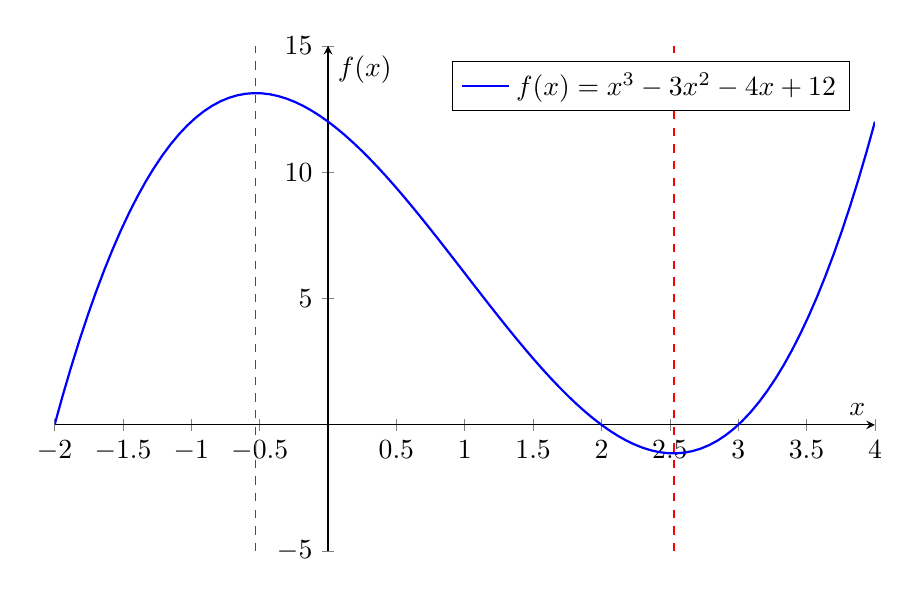
\begin{tikzpicture}
    \begin{axis}[
        axis lines = middle,
        xlabel = \(x\),
        ylabel = {\(f(x)\)},
        domain = -2:4,
        ymin = -5,
        ymax = 15,
        samples = 100,
        % grid = both,
        % minor tick num = 4,
        % major grid style = {lightgray},
        % minor grid style = {lightgray!25},
        width = 12cm,
        height = 8cm,
        legend pos = north east
    ]
    
    % Plot the cubic polynomial
    \addplot[blue, thick, no markers] {x^3 - 3*x^2 - 4*x + 12};
    \addlegendentry{\(f(x) = x^3 - 3x^2 - 4x + 12\)}

    % Draw vertical lines to partition the plot into monotonic sections
    \addplot[dashed, red] coordinates {(-0.53, -5) (-0.53, 15)};
    \addplot[dashed, red] coordinates {(2.53, -5) (2.53, 15)};
    
    % Add labels to indicate the partitions
    \node[above, red] at (axis cs: -0.53, 15) {\(x_1\)};
    \node[above, red] at (axis cs: 2.53, 15) {\(x_2\)};
    
    \end{axis}
\end{tikzpicture}

\end{document}
